\documentclass[10pt,a4paper, margin=1in]{article}
\usepackage{fullpage}
\usepackage{amsfonts, amsmath, pifont}
\usepackage{amsthm}
\usepackage{graphicx}
\usepackage{fullpage}
\usepackage{amsfonts, amsmath, pifont}
\usepackage{amsthm}
\usepackage{graphicx}
\usepackage{float}

\usepackage{tkz-euclide}
\usepackage{tikz}
\usepackage{pgfplots}
\pgfplotsset{compat=1.13}
\usepackage[utf8]{inputenc}



\usepackage{geometry}
 \geometry{
 a4paper,
 total={210mm,297mm},
 left=10mm,
 right=10mm,
 top=10mm,
 bottom=16mm,
 }
 \begin{filecontents}{q5_odd_new_.dat}
 n   xn 
 -8  0
 -7   -1.5
 -6   0
 -5   0
 -4   2
 -3   0 
 -2   -1
 -1   0.5
 0   0
 1   -0.5
 2   1
 3   0
 4   -2 
 5   0
 6   0
 7   1.5
 8   0
\end{filecontents}

\begin{filecontents}{q5_even_new_.dat}
 n   xn 
 -8  0
 -7   1.5
 -6   0
 -5   0
 -4   -2
 -3   0 
 -2   1
 -1   -0.5
 0   0
 1   -0.5
 2   1
 3   0
 4   -2 
 5   0
 6   0
 7   1.5
 8   0
\end{filecontents}

\begin{filecontents}{q3_a.dat}
 n   xn 
 -8  0
 -7  3
 -6   0
 -5   0
 -4   -4
 -3   0 
 -2   2
 -1   -1
 0   -1
 1   0
 2   0
 3   3
 4   0 
\end{filecontents}


 
 % Write both of your names here. Fill exxxxxxx with your ceng mail address.
 \author{
  Düzel, Uğur\\
  \texttt{e2171569@ceng.metu.edu.tr}
  \and
  Yalçınkaya, Beyazıt\\
  \texttt{e2172138@ceng.metu.edu.tr}
}
\title{CENG 384 - Signals and Systems for Computer Engineers \\
Spring 2018-2019 \\
Written Assignment 1}
\begin{document}
\maketitle



\noindent\rule{19cm}{1.2pt}

\begin{enumerate}

\item 
    \begin{enumerate}
    % Write your solutions in the following items.
    \item %write the solution of q1a
    	First, let's put value of $z$ form the first equation to the second equation. Notice that the conjugate of $z$ is $\bar{z} = x -yj$. Then, we solve the equation to find values of $x$ and $y$.
    	\begin{equation}
	\begin{split}
		3z + 4 & = 2j - \bar{z}\\
		3(x + yj) + 4 & = 2j - (x - yj)\\
		3x + 3yj + 4 & = 2j - x + yj\\
		4x + 2yj - 2j & = -4\\
		4x + 2j(y - 1) & = -4\\
		x & = -1\\
		y & = 1
	\end{split}
	\end{equation}
	
	\begin{itemize}
		\item[(i)] Below, we find $|z|^2$.
            		\begin{equation}
	       	 	\begin{split}
        				|z|^2 & = x^2 + y^2\\
        				|z|^2 & = (-1)^2 + (1)^2\\
        				|z|^2 & = 2
	        		\end{split}
       		 	\end{equation}
		\item[(ii)] Below, we plot $z$ on the complex plane.

\begin{figure}[!htbp]
\begin{center}
\begin{tikzpicture}
    \begin{scope}[thick,font=\scriptsize]
    
    
    \draw [->] (-4,0) -- (4,0) node [above left]  {$\Re\{z\}$};
    \draw [->] (0,-4) -- (0,4) node [below right] {$\Im\{z\}$};

    
    \foreach \n in {-3,...,-1,1,2,...,3}{%
        \draw (\n,-3pt) -- (\n,3pt)   node [above] {$\n$};
        \draw (-3pt,\n) -- (3pt,\n)   node [right] {$\n i$};}
        
    \draw [thick, color=red] (0,0) -- (-1,1);
    \draw [color=blue, fill=blue] (-1,1) circle(0.05);
    \node [color=black] at (-1,1.3) {$ -1+i$};
\end{scope}
\end{tikzpicture}
\end{center}
\caption{ \textit{\textbf{$z=-1+i$}} is plotted on on the Complex Plane}
\end{figure}
		
	\end{itemize}
    
    \item %write the solution of q1b
    Since $z^3=64j$, $z=-4j$. Below, we find $z$ in polar form.
	\begin{equation}
	\begin{split}
		\Theta & = \tan^{-1}{\left( \frac{b}{a} \right)} = \tan^{-1}{\left( \frac{-4}{0} \right)} = \frac{-\pi}{2} \\
		r & = \sqrt{a^2+b^2} = \sqrt{0^2+4^2} = 4 \\
		z & = 4e^{j\frac{-\pi}{2}} \\
		& = 4\left( \cos{\left( \frac{-\pi}{2} \right)}+j\sin{\left( \frac{-\pi}{2} \right)} \right) \\
		& = 4j\sin{\left( \frac{-\pi}{2} \right)}
	\end{split}
	\end{equation}
    
    \item %write the solution of q1c
    Below, we find the magnitude and angle of $z$.
	\begin{equation}
	\begin{split}
		z & = \frac{(1-j)(1+\sqrt{3}j)}{(1+j)} \\
		& = \frac{(1-j)(1-j)(1+\sqrt{3}j)}{(1+j)(1-j)} \\
		& = \frac{(-2j)(1+\sqrt{3}j)}{2} \\ 
		& = -j(1+\sqrt{3}j) \\
		& = -j+\sqrt{3} \\ 
		r & = \sqrt{a^2+b^2} = \sqrt{1+3} = 2 \\
		\Theta & = \tan^{-1}{\left( \frac{b}{a} \right)} = \tan^{-1}{\left( \frac{-1}{\sqrt{3}} \right)} = \frac{-\pi}{6}
	\end{split}
	\end{equation}
    \item %write the solution of q1d
    Below, we write $z$ in polar form.
	\begin{equation}
	\begin{split}
		z & = -je^{j\frac{\pi}{2}}\\
		z &  = -j\left( \cos{\left( \frac{\pi}{2} \right)} + j\sin{\left( {\frac{\pi}{2}} \right)}\right)\\
		z &  = 1\\
		z & = \cos{\left( 0 \right)}
	\end{split}
	\end{equation}
    	
    \end{enumerate}


\item %write the solution of q2
You can see the graph in Figure 2.
     \begin{figure}[H]
    \centering
        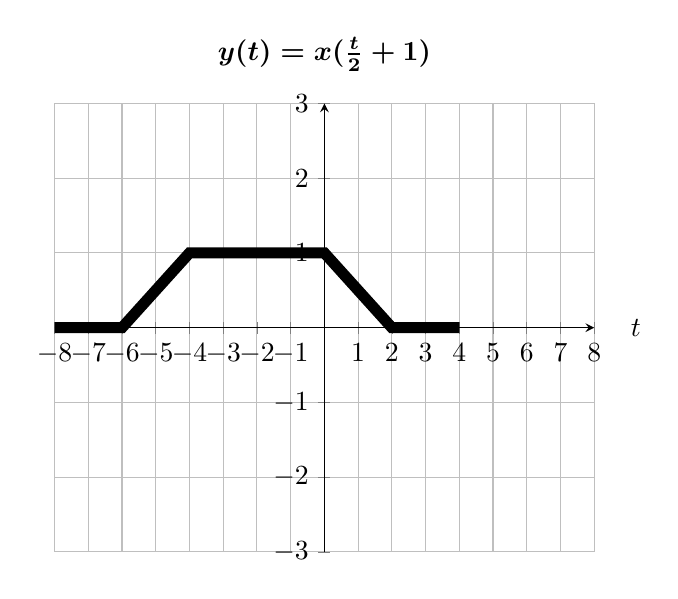
\begin{tikzpicture}[scale=1.0]
           \begin{axis}[
          axis lines=middle,
          xlabel={$t$},
          ylabel={$\boldsymbol{y(t)=x(\frac{t}{2}+1)}$},
          xtick={-8, -7, ..., 8},
          ytick={-3, -2, -1, ..., 3},
          ymin=-3, ymax=3,
          xmin=-8, xmax=8,
          every axis x label/.style={at={(ticklabel* cs:1.05)}, anchor=west,},
          every axis y label/.style={at={(ticklabel* cs:1.05)}, anchor=south,},
          grid,
        ]
           %\path[draw,line width=4pt] (-7,0) -- (-5,0) -- (-3,1) -- (1,1) -- (3,0) -- (5,0);
           \path[draw,line width=4pt] (-8,0) -- (-6,0) -- (-4,1) -- (0,1) -- (2,0) -- (4,0);
           \end{axis}
        \end{tikzpicture}
        \caption{$t$ vs. $y(t)=x(\frac{t}{2}+1)$.}
        \label{fig:q2}
    \end{figure}
    
   
    
\item      
    \begin{enumerate}
    \item %write the solution of q3a
    The graph can be seen in Figure 3. \\
    \begin{figure} [H]
    \centering
    \begin{tikzpicture}[scale=1.0] 
      \begin{axis}[
          axis lines=middle,
          xlabel={$n$},
          ylabel={$\boldsymbol{x[-n]+x[2n+1]}$},
          xtick={ -8, -7, ..., 4},
          ytick={-4, -3, -2, -1, ..., 4},
          ymin=-4, ymax=4,
          xmin=-8, xmax=4,
          every axis x label/.style={at={(ticklabel* cs:1.05)}, anchor=west,},
          every axis y label/.style={at={(ticklabel* cs:1.05)}, anchor=south,},
          grid,
        ]
        \addplot [ycomb, black, thick, mark=*] table [x={n}, y={xn}] {q3_a.dat};
      \end{axis}
    \end{tikzpicture}
    \caption{$n$ vs. $x[-n]+x[2n+1]$.}
    \label{fig:q3}
\end{figure}

    \item %write the solution of q3b
    Below, we present $x[-n] + x[2n+1]$ in terms of the unit impulse function.
	\begin{equation}
	\begin{split}
		x[n] & = -\delta[n - 1] + 2\delta[n - 2] -4\delta[n-4] + 3\delta[n-7]\\
		x[-n] & = -\delta[-n - 1] + 2\delta[-n - 2] -4\delta[-n-4] + 3\delta[-n-7]\\
		x[2n+1] & = -\delta[2n] + 2\delta[2n - 1] -4\delta[2n - 3] + 3\delta[2n - 6]\\
		x[-n] + x[2n+1] & = -\delta[-n - 1] + 2\delta[-n - 2] -4\delta[-n-4] + 3\delta[-n-7]\\
		& \qquad \qquad \qquad - \delta[2n] + 2\delta[2n - 1] -4\delta[2n - 3] + 3\delta[2n - 6]\\
		x[-n] + x[2n+1] & = -\delta[n + 1] + 2\delta[n + 2] -4\delta[n + 4] + 3\delta[n + 7] - \delta[n] + 3\delta[n - 3]
	\end{split}
	\end{equation}
    
    \end{enumerate}

\item 
    \begin{enumerate}
    \item %write the solution of q4a
    	In this question, we will find the periods of the $\sin$ and $\cos$ functions separately and then we will find the period of the whole function.
	
	A signal in the form of $A\cos{[\Omega_0 n + c]}$ where $c$ is a real number is periodic if $\frac{\Omega_0}{2 \pi} = \frac{m}{N_0}$ and $m$ and $N_0$ are integers. Moreover, the smallest integer value of $N_0$ is the fundamental period. For the given signal $3\cos{[\frac{13 \pi}{10} n]}$, we have $\frac{\frac{13 \pi}{10}}{2 \pi} = \frac{13}{20} = \frac{m}{N_0}$. For $m = 13$, $N_0 = 20$. Notice that $m = 13$ is the smallest integer value of $m$ that makes $N_0$ an integer. Hence, the signal is periodic with the fundamental period $N_0 = 20$.
	
	A signal in the form of $A\sin{[\Omega_0 n + c]}$ where $c$ is a real number is periodic if $\frac{\Omega_0}{2 \pi} = \frac{m}{N_0}$ and $m$ and $N_0$ are integers. Moreover, the smallest integer value of $N_0$ is the fundamental period. For the given signal $5\sin{[\frac{7 \pi}{3} n - \frac{2 \pi}{3}]}$, we have $\frac{\frac{7 \pi}{3}}{2 \pi} = \frac{7}{6} = \frac{m}{N_0}$. For $m = 7$, $N_0 = 6$. Notice that $m = 7$ is the smallest integer value of $m$ that makes $N_0$ an integer. Hence, the signal is periodic with the fundamental period $N_0 = 6$.
	
	Now, we have two signals with fundamental periods $20$ and $6$, i.e., the first signal repeats itself for $n = 20, 40, \underline{60}, 80, \ldots$ and the second signal repeats itself for $n = 6, 12, 18, 24, 30, 36, 40, 44, 48, 52, 56, \underline{60}, \ldots$. The summation of these signals is a new signal which repeats itself for $n = \underline{60}, 120, \ldots$. Hence, the signal $3\cos{[\frac{13 \pi}{10} n]} + 5\sin{[\frac{7 \pi}{3} n - \frac{2 \pi}{3}]}$ is periodic with the fundamental period $N_0 = 60$.
    
    
    
    \item %write the solution of q4b
    	A signal in the form of $A\sin{[\Omega_0 n + c]}$ where $c$ is a real number is periodic if $\frac{\Omega_0}{2 \pi} = \frac{m}{N_0}$ and $m$ and $N_0$ are integers. Moreover, the smallest integer value of $N_0$ is the fundamental period. For the given signal $5\sin{[3n - \frac{\pi}{4}]}$, we have $\frac{3}{2 \pi} = \frac{m}{N_0}$. There is no integer value of $m$ that makes $N_0$ an integer. Hence, the given signal is not periodic.
    \item %write the solution of q4c
    	A signal in the form of $A\cos{(\omega_0 t + c)}$ where $c$ is a real number is periodic with the fundemental period $T_0 = \frac{2 \pi}{\omega_0}$ where $T_0$ is a real number. For the given signal $2\cos{(3 \pi t - \frac{2 \pi}{5})}$, we have $T_ 0 = \frac{2}{3}$. Hence, the given signal is periodic with the fundamental period $T_0 = \frac{2}{3}$.
	
    \item %write the solution of q4d
    In this question, we solve the equation $x(t) = x(t + T)$ in order to find the period $T$.

    	\begin{equation}
	\begin{split}
		x(t) & = x(t + T)\\
		-je^{j5t} & = -je^{j5(t + T)}\\
		e^{j5t} & = e^{j5(t + T)}\\
		e^{j5t} & = e^{j5t} e^{j5T}\\
		1 & = e^{j5T} = \cos{(5T)} + \sin{(5T)}\\
		2 \pi & = 5T\\
		T_0 & = \frac{2 \pi}{5}
	\end{split}
	\end{equation}
    	Notice that, since $5T = 0$ is the trivial solution, we pick the next smallest value $5T = 2 \pi$ to find the fundamental period. Hence, the given signal is periodic with the fundamental period $T_0 = \frac{2 \pi}{5}$
    \end{enumerate}

\item %write the solution of q5
First, we check whether $x[n]$ is odd or even or none. For oddness, we check whether $x[n] = - x[-n]$ holds and for evenness, we check whether $x[n] = x[-n]$ holds.
	\begin{itemize}
		\item[(i)] Oddness:
			\begin{equation}
			\begin{split}
				-\delta[n - 1] + 2\delta[n - 2] -4\delta[n-4] + 3\delta[n-7] \not= \delta[-n - 1] - 2\delta[-n - 2] + 4\delta[-n-4] - 3\delta[-n-7]
			\end{split}
			\end{equation}
		\item[(ii)] Evenness:
			\begin{equation}
			\begin{split}
				-\delta[n - 1] + 2\delta[n - 2] -4\delta[n-4] + 3\delta[n-7] \not= -\delta[-n - 1] + 2\delta[-n - 2] - 4\delta[-n-4] + 3\delta[-n-7]
			\end{split}
			\end{equation}
	\end{itemize}
	
Hence, $x[n]$ is neither an odd nor an even function. Now, find the even and odd decompositions of $x[n]$ and give the graphs of both.
	\begin{itemize}
		\item[(i)] Oddness:
			\begin{equation}
			\begin{split}
				Odd\{x[n]\} & = \frac{1}{2} \left\{ x[n] - x[-n] \right\}\\
				& = \frac{1}{2} \left\{ -\delta[n - 1] + 2\delta[n - 2] -4\delta[n-4] + 3\delta[n-7] + \delta[-n - 1] - 2\delta[-n - 2] + 4\delta[-n-4] - 3\delta[-n-7] \right\}
			\end{split}
			\end{equation}
		\item[(ii)] Evenness:
			\begin{equation}
			\begin{split}
				Ev\{x[n]\} & = \frac{1}{2} \left\{ x[n] + x[-n] \right\}\\
				& = \frac{1}{2} \left\{ -\delta[n - 1] + 2\delta[n - 2] -4\delta[n-4] + 3\delta[n-7] - \delta[-n - 1] + 2\delta[-n - 2] - 4\delta[-n-4] + 3\delta[-n-7] \right\}
			\end{split}
			\end{equation}
	\end{itemize}





\begin{figure} [H]
    \centering
    \begin{tikzpicture}[scale=1.0] 
      \begin{axis}[
          axis lines=middle,
          xlabel={$n$},
          ylabel={$\boldsymbol{x[n]}$},
          xtick={ -8, -7, ..., 8},
          ytick={-4, -3, -2, -1, ..., 4},
          ymin=-4, ymax=4,
          xmin=-8, xmax=8,
          every axis x label/.style={at={(ticklabel* cs:1.05)}, anchor=west,},
          every axis y label/.style={at={(ticklabel* cs:1.05)}, anchor=south,},
          grid,
        ]
        \addplot [ycomb, black, thick, mark=*] table [x={n}, y={xn}] {q5_odd_new_.dat};
      \end{axis}
    \end{tikzpicture}
    \caption{$n$ vs. $Odd\{x[n]\}$.}
    \label{fig:q5}
\end{figure}

\begin{figure} [H]
    \centering
    \begin{tikzpicture}[scale=1.0] 
      \begin{axis}[
          axis lines=middle,
          xlabel={$n$},
          ylabel={$\boldsymbol{x[n]}$},
          xtick={ -8, -7, ..., 8},
          ytick={-4, -3, -2, -1, ..., 4},
          ymin=-4, ymax=4,
          xmin=-8, xmax=8,
          every axis x label/.style={at={(ticklabel* cs:1.05)}, anchor=west,},
          every axis y label/.style={at={(ticklabel* cs:1.05)}, anchor=south,},
          grid,
        ]
        \addplot [ycomb, black, thick, mark=*] table [x={n}, y={xn}] {q5_even_new_.dat};
      \end{axis}
    \end{tikzpicture}
    \caption{$n$ vs. $Ev\{x[n]\}$.}
    \label{fig:q5}
\end{figure}



\item 
    \begin{enumerate}
    \item %write the solution of q6a
    	
	\begin{itemize}
		\item \textbf{\textit{Memory:}} The system requires memory since the output value of the system depends on the value of $x(t)$ in a different time instance, e.g. $y(1) = x(-1)$.
		\item \textbf{\textit{Stability:}} The system is bounded because for bounded $x(t)$, $y(t)$ is bounded.
		\begin{equation}
		\begin{split}
			& -B < x(t) < B \\
			& -B < x(2t-3) < B \\
			& -B < y(t) < B 
		\end{split}
		\end{equation}
		\item \textbf{\textit{Causality:}} For $t = 4$, $y(4) = x(5)$ which violates the causality property; hence, the system is not causal.
		\item \textbf{\textit{Linearity:}} Consider two arbitrary inputs $x_1(t)$ and $x_2(t)$.
		\begin{equation}
		\begin{split}
			x_1(t) & \rightarrow y_1(t) = x_1(2t-3)\\
			x_2(t) & \rightarrow y_2(t) = x_2(2t-3)
		\end{split}
		\end{equation}
		Then, consider a linear combination of $x_1(t)$ and $x_2(t)$, i.e., $x_3(t)=\alpha x_1(t) + \beta x_2(t)$
		\begin{equation}
		\begin{split}
			y_3(t) & = x_3(2t - 3)\\
			& = \alpha x_1(2t-3) + \beta x_2(2t-3)\\
			& = \alpha y_1(t) + \beta y_2(t)
		\end{split}
		\end{equation}
		Therefore the system is linear.
		\item \textbf{\textit{Invertibility:}} When $x(t)$ is given to the system as the input, $y(t) = x(2t - 3)$ is the output. The inverse system takes $y(t)$ as the input and produces $w(t)$ as the output which should be equal to $x(t)$ in order system to be invertible. To ensure that $w(t)=y(\frac{t+3}{2})$ which produces $x(t)$. To prove that say $k=\frac{t+3}{2}$ then $y(k)=x(2k-3)$. Hence, the system is invertible since the invertible system exists.

		\item \textbf{\textit{Time-Invariance:}} Shift the input signal $x(t)$ by $t_0$, i.e., $x(t-t_0)$. When the shifted input is applied to the system, we get the following output signal $y(t-t_0)  = x(2t-2t_0-3)$. A time shift in the input signal does not result in an identical time shift in the output signal, i.e., $x(2t-2t_0-3) \neq x(2t - t_0 - 3)$. Hence, the system is not time invariant.
	\end{itemize}
    
    
    \item %write the solution of q6b
	\begin{itemize}
		\item \textbf{\textit{Memory:}} The system is memoryless since the output value of the system depends on the value of $x(t)$ in the current time instance for all values of $t$.
		\item \textbf{\textit{Stability:}} To disprove stability of this system we observe the following: a constant input $x(t)=1$ yields to $y(t)=t$ which is unbounded. Therefore, the system is not stable.
		\item \textbf{\textit{Causality:}} The system is causal since $y(t)$ only depends on the values of $x(t)$ at the current time instance.
		\item \textbf{\textit{Linearity:}} Consider two arbitrary inputs $x_1(t)$ and $x_2(t)$.
		\begin{equation}
		\begin{split}
			x_1(t) & \rightarrow y_1(t) = t x_1(t)\\
			x_2(t) & \rightarrow y_2(t) = t x_2(t)
		\end{split}
		\end{equation}
		Then, consider a linear combination of $x_1(t)$ and $x_2(t)$, i.e., $x_3(t)=\alpha x_1(t) + \beta x_2(t)$
		\begin{equation}
		\begin{split}
			y_3(t) & = t x_3(t)\\
			& = t (\alpha x_1(t) + \beta x_2(t))\\
			& = t\alpha x_1(t) + t\beta x_2(t)\\
			& = \alpha y_1(t) + \beta y_2(t)
		\end{split}
		\end{equation}
		Therefore the system is linear.
		\item \textbf{\textit{Invertibility:}} When $x(t)$ is given to the system as the input, $y(t) = tx(t)$ is the output. The inverse system takes $y(t)$ as the input and produces $w(t)$ as the output which should be equal to $x(t)$ in order system to be invertible. To ensure that $w(t)=\frac{y(t)}{t}$ which produces $x(t)$. To prove that observe $w(t) = \frac{y(t)}{t} = \frac{tx(t)}{t} = x(t)$. Hence, the system is invertible since the invertible system exists.
		
		
		
		\item \textbf{\textit{Time-Invariance:}} Shift the input signal $x(t)$ by 
		$t_0$, i.e., $x(t-t_0)$. When the shifted input is applied to the system, we get the following output signal $y(t-t_0)  = (t - t_0)x(t - t_0)$. A time shift in the input signal does not result in an identical time shift in the output signal, i.e., $(t - t_0)x(t - t_0) \neq tx(t - t_0)$. Hence, the system is not time invariant.
		
	\end{itemize}
    \item %write the solution of q6c
	\begin{itemize}
		\item \textbf{\textit{Memory:}} The system requires memory since the output value of the system depends on the value of $x[n]$ in a different time instance, e.g. $y[1] = x[-1]$.
		\item \textbf{\textit{Stability:}} The system is bounded because for bounded $x[n]$, $y[n]$ is bounded.
		\begin{equation}
		\begin{split}
			& -B < x[n] < B \\
			& -B < x[2n-3] < B \\
			& -B < y[n] < B 
		\end{split}
		\end{equation}
		\item \textbf{\textit{Causality:}} For $n = 4$, $y[4] = x[5]$ which violates the causality property; hence, the system is not causal.
		\item \textbf{\textit{Linearity:}} Consider two arbitrary inputs $x_1[n]$ and $x_2[n]$.
		\begin{equation}
		\begin{split}
			x_1[n] & \rightarrow y_1[n] = x_1[2n-3]\\
			x_2[n] & \rightarrow y_2[n] = x_2[2n-3]
		\end{split}
		\end{equation}
		Then, consider a linear combination of $x_1[n]$ and $x_2[n]$, i.e., $x_3[n]=\alpha x_1[n] + \beta x_2[n]$
		\begin{equation}
		\begin{split}
			y_3[n] & = x_3[2n - 3]\\
			& = \alpha x_1[2n - 3] + \beta x_2[2n - 3]\\
			& = \alpha y_1[n] + \beta y_2[n]
		\end{split}
		\end{equation}
		Therefore the system is linear.
		\item \textbf{\textit{Invertibility:}} Consider the inputs $x_1[n]=u[n]$ and $x_2[n]=u[n-1]$ where $u[n]$ is the unit step function. These inputs yield to $y_1[n]=x_1[2n-3]=u[2n-3]$ and $y_2[n]=x_2[2n-3]=u[2n-4]$ which implies $u[2n-3]=u[2n-4]=u[n-2]$ for all integer values of $n$. Hence, $y_1[n]=y_2[n]$ even though $x_1[n]\neq x_2[n]$ , therefore the system is not invertible since distinct inputs yield to the same outputs.
		
		%When $x[n]$ is given to the system as the input, $y[n] = x[2n - 3]$ is the output. The inverse system takes $y[t]$ as the input and produces $w[t]$ as the output which should be equal to $x[n]$ in order system to be invertible. To ensure that $w[n]=y[\frac{n+3}{2}]$ which produces $x[n]$. To prove that say $k=\frac{t+3}{2}$ then $y[k]=x[2k-3]$. Hence, the system is invertible since the invertible system exists.
		\item \textbf{\textit{Time-Invariance:}} Shift the input signal $x[n]$ by $n_0$, i.e., $x[n-n_0]$. When the shifted input is applied to the system, we get the following output signal $y[n-n_0]  = x[nt-nt_0-3]$. A time shift in the input signal does not result in an identical time shift in the output signal, i.e., $x[2n-2n_0-3] \neq x[2n - n_0 - 3]$. Hence, the system is not time invariant.
	\end{itemize}
    \item %write the solution of q6d
	\begin{itemize}
		\item \textbf{\textit{Memory:}} The system requires memory since the output value of the system depends on the value of $x[n]$ in different time instances, e.g. $y[1] = x[0] + x[-1] + \ldots$.
		\item \textbf{\textit{Stability:}} 
			To disprove stability of the system observe the following: a constant input $x[n]=1$ yields to $y[n]=\sum_{k=1}^{\infty} 1$ which does not converge to value; hence, is unbounded. Therefore, the system is not stable.	
		
		
		
		%The system is bounded because for bounded $x[n]$, $y[n]$ is bounded.
		%\begin{equation}
		%\begin{split}
		%	-B <& x[n] < B \\
		%	-B <& x[n-k] < B \\
		%	\sum_{k=1}^{\infty} -B <& \sum_{k=1}^{\infty} x[n-k] < \sum_{k=1}^{\infty} B \\
		%	-\infty <& y[n] < \infty
		%\end{split}
		%\end{equation}
		\item \textbf{\textit{Causality:}} The system is causal since the output only depends on the values of the input in the past.
		\item \textbf{\textit{Linearity:}} Consider two arbitrary inputs $x_1[n]$ and $x_2[n]$.
		\begin{equation}
		\begin{split}
			x_1[n] & \rightarrow y_1[n] = \sum_{k=1}^{\infty}x_1[n-k]\\
			x_2[n] & \rightarrow y_2[n] = \sum_{k=1}^{\infty}x_2[n-k]
		\end{split}
		\end{equation}
		Then, consider a linear combination of $x_1[n]$ and $x_2[n]$, i.e., $x_3[n]=\alpha x_1[n] + \beta x_2[n]$
		\begin{equation}
		\begin{split}
			y_3[n] & = \sum_{k=1}^{\infty}x_3[n-k]\\
			y_3[n] & = \sum_{k=1}^{\infty} \left( \alpha x_1[n - k] + \beta x_2[n - k] \right)\\
			y_3[n] & = \sum_{k=1}^{\infty} \alpha x_1[n - k] + \sum_{k=1}^{\infty} \beta x_2[n - k]\\
			& = \alpha \sum_{k=1}^{\infty}x_1[n-k] + \beta \sum_{k=1}^{\infty}x_2[n-k]\\
			& = \alpha y_1[n] + \beta y_2[n]
		\end{split}
		\end{equation}
		Therefore the system is linear.
		\item \textbf{\textit{Invertibility:}}  When $x[n]$ is given to the system as the input, $y[n] = \sum_{k=1}^{\infty} x[n-k]$ is the output. The inverse system takes $y[n]$ as the input and produces $w[n]$ as the output which should be equal to $x[n]$ in order system to be invertible. To ensure that $w[n]=y[n+1]-y[n]$ which produces $x[n]$. To prove that observe the following $y[n+1]= \sum_{k=1}^{\infty} x[n-k+1]$ and $y[n] = \sum_{k=1}^{\infty} x[n-k] = \sum_{k=2}^{\infty} x[n-k+1]$ so $y[n+1]-y[n]=x[n]$. Hence, the system is invertible since the invertible system exists.
		\item \textbf{\textit{Time-Invariance:}} Shift the input signal $x[n]$ by $n_0$, i.e., $x[n-n_0]$. When the shifted input is applied to the system, we get the following output signal $\sum_{k=1}^{\infty}x[n-n_0-k]$. To prove time invariance observe the following argument $\sum_{k=1}^{\infty}x[n-n_0-k] = \sum_{l=1+n_0}^{\infty}x[n-l] = y[n-n_0]$. Hence, the system is time invariant.
	\end{itemize}
    \end{enumerate}

\end{enumerate}
\end{document}

